%We describe the problem statement, the approach, the dataset, and the main experimental results of AppEvolve.

\subsection{Problem Statement}\label{sec:problem}
%Consider two Android API versions: $oldAPIs = [m_1, m_2, ..., m_k]$ and $newAPIs = [m_1', m_2', ..., m_l']$. An API usage may involve one or more methods from either $oldAPIs$ or $newAPIs$. An API usage change from the $oldAPIs$ to the $newAPIs$ can be defined as a change from one or more methods from the $oldAPIs$ to one or more methods from the $newAPIs$, which can be written as $[m_1, m_2, ..., m_p] \rightarrow [m_1', m_2', ..., m_q']$. The goal of automatic update of Android apps is to update usages of $oldAPIs$ to $newAPIs$ based on the API usage change while also maintaining backward compatibility.

AppEvolve targets the case where a set of one or more API methods of
the Android framework are deprecated by another set of one or more
API methods in a new version of the framework and the Android apps that use the old APIs need to be updated.
The goal of AppEvolve is to
automatically update such Android apps so that they use
the new APIs, while maintaining backward compatibility.

%\begin{figure*}[htb]
%	\centering
%	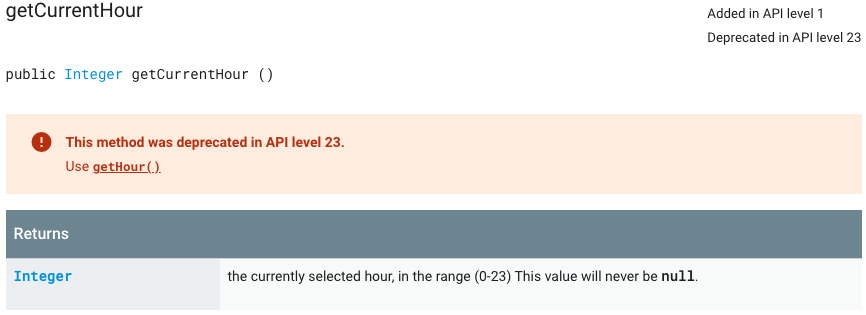
\includegraphics[width=0.8\linewidth]{deprecated-api-example.png}
%	\caption{An example of a deprecated API
%	}
%	\label{fig:deprecated_api_example}
%\end{figure*}

To illustrate the API usage update problem, consider a change in the
Android API: the method \texttt{getCurrentHour()} was added in the Android API version 1 to return
the current hour; it was deprecated in the version 23 of the Android API and the
method \texttt{getHour()} was suggested as its replacement.

Figure~\ref{fig:deprecated_api_update_example} shows an example of an API
usage change that modifies a usage of method \texttt{getCurrentHour()} to
its replacement method \texttt{getHour()}. Given this example, one can possibly
learn a generic patch as shown in
Figure~\ref{fig:deprecated_api_update_edits}. The generic patch updates a
deprecated method usage to a replacement method usage.
Backward compatibility is achieved by checking the version number of the
mobile OS running the app. If the version is greater than or equal to a
certain version number, the replacement method is used. Otherwise, the
deprecated method is used.

\begin{figure}[htb]
\centering
\begin{lstlisting}[language=diff,numbers=none]
private long addEventToGCal() {
  ...
  int hourInt;
  int minInt;
- hourInt = timepicker.getCurrentHour();
- minInt = timepicker.getCurrentMinute();
+ if (android.os.Build.VERSION.SDK_INT >=
+       android.os.Build.VERSION_CODES.M) {
+  hourInt = timepicker.getHour();
+  minInt = timepicker.getMinute();
+ } else {
+  hourInt = timepicker.getCurrentHour();
+  minInt = timepicker.getCurrentMinute();
+ }
  ...
}
\end{lstlisting}
\caption{A deprecated API-usage update}
\label{fig:deprecated_api_update_example}
\end{figure}

\begin{figure}[htb]
\centering
\begin{lstlisting}[language=diff,numbers=none]
- $T2 = $T1.getCurrentHour();
+ if (android.os.Build.VERSION.SDK_INT >=
+       android.os.Build.VERSION_CODES.M) {
+  $T2 = $T1.getHour();
+ } else {
+  $T2 = $T1.getCurrentHour();
+ }
\end{lstlisting}
\caption{A generic patch for updating uses of \texttt{getCurrentHour()}}
\label{fig:deprecated_api_update_edits}
\end{figure}

\jl{Figure \ref{fig:deprecated_api_update_edits} uses $-$ and $+$, but the
  AppEvolve paper uses I M D and U.}

\subsection{Approach}
\toolname\ takes as input a target app to update and a mapping from
deprecated API method(s) to the corresponding replacement API method(s).
AppEvolve is divided into four phases: {\em API-Usage Analysis}, {\em
  Update Example Search}, {\em Update Example Analysis} and {\em API-Usage
  Update}, as shown in Figure~\ref{fig:framework}.

In the {\em API-Usage Analysis} phase, \toolname\ accepts as input an {\em
  API Usage Change} and a {\em Target App}. An {\em API Usage Change}
describes the mapping from the deprecated API method(s) to the
corresponding replacement API method(s).  Information about this API Usage
Change may come, for example, from the documentation of the API itself. A
{\em Target App} is an app that contains a usage of the deprecated API
method and requires updates to make use of the replacement API
method. Given these two inputs, \toolname\ pinpoints the location of the
deprecated API usage in the {\em Target App}. In the {\em Update Example
  Search} phase, \toolname\ searches GitHub for examples of API usage
updates that modify the usage of the deprecated API method to include the
usage of the replacement API methods. In the {\em Update Example Analysis}
phase, \toolname\ generates generic patches from the examples of API usage
updates and ranks these patches. In the {\em API Usage Update} phase,
\toolname\ tries to apply the ranked patches one by one and returns the
                 {\em Evolved Target App} if any of the edits is successful
                 and validated.

\begin{figure*}[t]
	\centering
	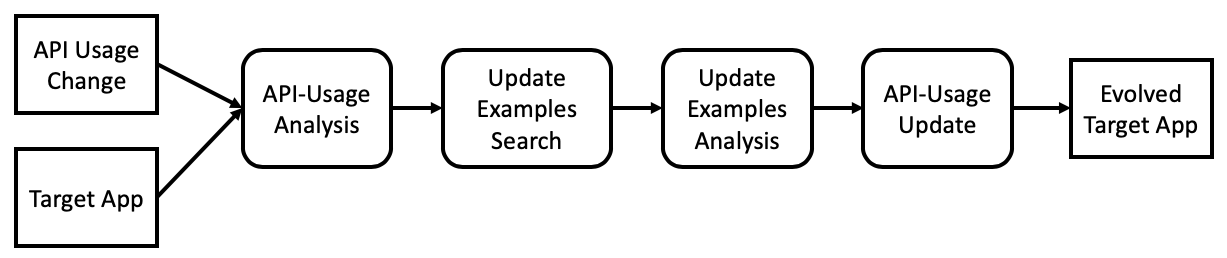
\includegraphics[width=0.8\linewidth]{framework.png}
	\caption{Framework of AppEvolve}
	\label{fig:framework}
\end{figure*}

We next describe each of the above phases in detail.
\subsubsection{API-Usage Analysis}
\toolname\ finds the location where the deprecated API method specified in
the {\em API Usage Change} is used inside the {\em Target App}. Consider
the deprecated API method \texttt{getCurrentHour()} mentioned in
Section~\ref{sec:problem}.  In this case, the {\em API Usage Change} is the
replacement of \texttt{getCurrentHour()} with \texttt{getHour()}. Given
this information, \toolname\ finds the location in the {\em Target App}
that invokes \texttt{getCurrentHour()}.

\subsubsection{Update Example Search}
\toolname\ searches for apps in GitHub that use both the deprecated and the
replacement API methods in their latest versions.  For each such app,
AppEvolve looks through the app history to find the commit where the uses
of the replacement API methods are added. This is intended to find examples
that produce a backward compatible Android app.  For each of these apps,
\toolname\ finds the changes that add the replacement API method to the app
code that already contains the deprecated API method. These changes are the
examples that can be used to update deprecated API method usages in other
apps.

\subsubsection{Update Example Analysis}
Given the examples found in GitHub, AppEvolve translates each example to a
generic patch. It does so by identifying edits related to the API usage via
intraprocedural forward and backward dependency analysis on the variables
involved in the API usage. Variables that are used in statements affected
by the edits but not defined by the edits themselves are considered as
context variables. All variables in the edits are then abstracted. Given
the generic patches, AppEvolve computes the common core of these generic
patches, defined as the longest subsequence of edits that are shared across
the patches. The generic patches are then ranked based on their distance to
the core.

\subsubsection{API-Usage Update}
Given a {\em Target App}, AppEvolve applies the generic patches according
to their computed rank in the previous phase. When applying a patch,
AppEvolve first finds mappings of the context variables to variables in the
{\em Target App}. For each such mapping, AppEvolve then tries to apply the
patch. If the edits are successfully applied, AppEvolve returns the {\em
  Evolved Target App}.

\subsection{Experiments}
For the target apps, the AppEvolve paper used 15 real-world apps from the
F-droid repository.\footnote{\url{https://fdroid.org}} These apps comprise
five apps for each of Android API versions 22, 23, and 25, and cover 20 API
usages in 41 locations. For each API version, the API change is manually
identified by reading the API documentation. Using the API change, the API
usage in each app is guaranteed to be: (1) different from the ones in the
other apps and (2) updated in the subsequent API version.  When applied to
the 15 apps considered, AppEvolve was able to update 17 out of 20 API
usages (85.00\% success rate) and 37 out of 41 of their occurrences across the
apps.

